%%%%%%%%%%%%%%%%%%%%%%%%%%%%%%%%%%%%%%%%%%%%%%%%%%%%%%%%%%%%%%%%%%%%%%%%%%%%%%%%
%2345678901234567890123456789012345678901234567890123456789012345678901234567890
%        1         2         3         4         5         6         7         8

\documentclass[letterpaper, 10 pt, conference]{ieeeconf}  % Comment this line out if you need a4paper

%\documentclass[a4paper, 10pt, conference]{ieeeconf}      % Use this line for a4 paper

\IEEEoverridecommandlockouts                              % This command is only needed if 
                                                          % you want to use the \thanks command

\overrideIEEEmargins                                      % Needed to meet printer requirements.

%In case you encounter the following error:
%Error 1010 The PDF file may be corrupt (unable to open PDF file) OR
%Error 1000 An error occurred while parsing a contents stream. Unable to analyze the PDF file.
%This is a known problem with pdfLaTeX conversion filter. The file cannot be opened with acrobat reader
%Please use one of the alternatives below to circumvent this error by uncommenting one or the other
%\pdfobjcompresslevel=0
%\pdfminorversion=4

% See the \addtolength command later in the file to balance the column lengths
% on the last page of the document

% The following packages can be found on http:\\www.ctan.org
%\usepackage{graphics} % for pdf, bitmapped graphics files
%\usepackage{epsfig} % for postscript graphics files
%\usepackage{mathptmx} % assumes new font selection scheme installed
%\usepackage{times} % assumes new font selection scheme installed
%\usepackage{amsmath} % assumes amsmath package installed
%\usepackage{amssymb}  % assumes amsmath package installed
\usepackage{graphicx}
\graphicspath{ {./images/} }
\usepackage{subcaption}
\usepackage{url}
\usepackage{booktabs}
\usepackage{hyperref}

\title{\LARGE \bf
Using Scene Graph Generation to Support LLM-Based Queries to a Vision System}


\author{Raghav Rangan, Siddh Bamb, Kevin Zhao, Zhongyan He% <-this % stops a space
}
%\thanks{*This work was supported by...}% <-this % stops a space
%\thanks{$^{1}$Christina Petlowany is with the Cockrell School of Engineering,
%        The University of Texas at Austin, Austin, TX 78712, USA
%        {\tt\small cpetlowany@utexas.edu}}%
%\thanks{$^{2}$Justin Hart is with the College of Natural Sciences, The %University of Texas at Austin,
%        Austin, TX 78712, USA
%        {\tt\small justinhart@utexas.edu}}%
%}

% todo other authors


\begin{document}



\maketitle
\thispagestyle{empty}
\pagestyle{empty}


%%%%%%%%%%%%%%%%%%%%%%%%%%%%%%%%%%%%%%%%%%%%%%%%%%%%%%%%%%%%%%%%%%%%%%%%%%%%%%%%
\begin{abstract}
    This work proposes the design and implementation of an LLM-based system to respond to queries regarding the state of a mapped space using labeled data regarding objects within the space. The goal of the system is to represent relationships between objects in order to answer semantic, positional, or quantificational queries regarding the mapped scene, or provide a general overview or summary when prompted. The system generates map data through the use of a scene graph generation (SGG) model. The output of this model, which is a relational graph connecting all the objects the network detects in the scene, is converted into a set of descriptive phrases via a graph traversal algorithm. These contextual descriptions are used by GPT-3.5 to analyze and respond to queries about the scene. The system is evaluated based on its accuracy and confidence in identifying relationships within unlabeled sample images as compared to correctly labeled versions of the same images. Results show that ChatGPT is capable of answering questions based on contextual information provided to it, and the SGG model was able to create detailed and accurate relational graphs of several test scenarios to provide the necessary phrases to ChatGPT to answer queries.
\end{abstract}
    
\section{Introduction}
    This paper proposes a system for an LLM-based image query system based on positional and semantic queries about objects in a scene. Vision-based queries are an important aspect of human-robot interaction which are key to facilitate collaboration between robots and humans and to allow robots to perform services for humans \cite{robinson2023vision}. Among other applications, semantic and relational querying systems can be used by service robots to assist visually impaired users with day-to-day tasks \cite{azenkot2016enabling}. This requires such querying systems to have sufficient accuracy and efficient performance to be feasible for use with service robots.

    Current models to identify object relations within a scene often have inaccuracies in their results or are computationally expensive to an extent which may be prohibitive to running them in real time. To identify the ability of existing models to address the task of responding to relational queries, an exploration of existing object detection frameworks, namely CLIP, was conducted with sample images and queries. It was found that image segmentation models perform poorly when identifying positional relationships, often detecting contradictory phrases with equal confidence or omitting important relationships. In order to achieve more accurate results, we considered a wider variety of object detection models which placed an emphasis on relational labeling, before deciding on scene graph generation (SGG) models.
    
    From end to end, an SGG model is capable of taking an input image, detecting objects within the image, and creating a graph that relates pairs of these objects. The vertices of this graph are the detected objects, and the edges connecting vertices represent the most confident relationship between them. Because SGG models are based on two-dimensional image detection rather than point cloud or voxel data, they may provide significant performance advantages over their three-dimensional counterparts, enabling additional use cases.
    
    We selected an SGG model trained on Visual Genome \cite{Krishna_Zhu_Groth_Johnson_Hata_Kravitz_Chen_Kalantidis_Li_Shamma_et_al._2017}, a dataset containing various images annotated with a relational graph of their contents. The edges of the output graph represent prepositions, thus drawing a positional relationship between a pair of objects. Converting the resultant graph into a set of phrases is accomplished by iterating through the pairs and appending to descriptor strings. The system provides this set of descriptions to ChatGPT through the GPT-3.5 API as context. Specifically, ChatGPT is prompted to answer following questions based on the provided context. Finally, the user is able to interact with the data, asking questions similar to, "How many chairs are in the room?", "Is there a lamp next to the sofa?", "Describe the left side of the room", etc.


\section{Related Works}
    
    Related models such as CLIP and CLIPSeg \cite{lueddecke22_cvpr} make use of joint embedding spaces to select text descriptions which match with the semantic content of an image, which can be of use to determine relationships in an image. Specifically, CLIP is a contrastive learning image model that takes advantage of a joint embedding space mapped onto by both a text encoder and image encoder~\cite{radford2021learning}. By training encoders to map semantically similar text and images to similar values and reject dissimilar ones, the model can then choose text which matches the image most accurately. This allows for impressive zero shot performance, much better than previous models like ImageNet. We initially provided the CLIP model with a list of object relationships to find in an input image, such as ``Person next to table',``Laptop on table', etc. Results showed that CLIP tends to perform poorly when inferring positional relationships between multiple objects in the frame as opposed to their presence in the image. Furthermore, descriptions where one object was present in the picture and the other wasn't created inconsistent outputs from the CLIP model.

    We also explored the accuracy of ChatGPT and other LLMs in identifying and answering queries about object relationships. Providing CLIP's top-20 outputs to ChatGPT showed that the LLM interface was very good at ``remembering' a set of information and answering queries regarding that information correctly. ChatGPT, on its own, is capable of correctly identifying details from provided relational context, and providing answers that were consistent with the body of information provided. This initial experiment proved the need for an alternative method to identify positional relationships between objects, and proved the viability of ChatGPT as a functional LLM interface to answer queries given a body of information.

    From these findings, we explored alternative techniques to identify inter-object relationships, including Scene Graph Generation (SGG) models, which specialize in representing positional relationships via edges on a graph. An early SGG model for inferring positional relationships is the Graph-RCNN network \cite{yang2018graph}, a model that builds on top of the Faster-RCNN object detection framework to allow for scene graph generation. The model uses a novel combination of a Relational Proposal Network, which handles predicting object relatedness, and a Graph Convolutional Network, which procedurally generates the output graph based on the object relations predicted by the RePN. The output is a refined, pruned graph, containing objects and their relevant relations. 
    
    Another, more modern SGG model, Neural Motifs \cite{zellers2018scenegraphs}, explored a different approach to SGG which focused on the fact that inter-object relations have a very repetitive nature, often remaining the same between identical objects in different scenes. The introduction of this idea allows for the model to predict these patterns or motifs across images, often correctly predicting edges that did not exist in provided ground-truth test images. 
    
    Finally, one of the current state-of-the-art SGG models is Causal-TDE, which has the highest recall@50 on the Visual Genome dataset \cite{latestinML}. This model attempts to solve one of the main issues in SGG, which is training bias. Due to more generic relations being more common in datasets, SGG models tend to predict more generic relations between things when they actually have the information to provide a more specific relation. For example, SGG models may prefer "Person on bike" over "Person riding on bike", a more specific prepositional phrase \cite{tang2020unbiased}. To counter this, the model makes two inferences, one considering the two objects (biased), and one with the two objects removed from the image (unbiased). Taking the difference in the predicted relation vectors between the two inferences, also known as Total Direct Effect (TDE) provides a more accurate and detailed relation between the objects \cite{tang2020unbiased}. The graph generation aspect of this model is implemented by a MotifNet \cite{zellers2018scenegraphs}, which is adapted to generate a causal graph and a counterfactual graph, the difference of which is taken as a final prediction. This Causal-TDE model has sufficient accuracy to find relationships between objects in an image, but cannot directly respond to queries about these relationships.



\section{Methodology}
    The propsed system takes the form of the following three-phase pipeline:
    \begin{itemize}
        \item The Scene Graph Generation (SGG) model to generate JSON format relational data
        \item Phrase Generation algorithm to convert output JSON into a context string
        \item ChatGPT interface to answer queries with information provided by the context string.
    \end{itemize}

    \subsection*{The SGG Model}
        The current system uses a pre-trained SGG Model, trained on the Visual Genome dataset. The model is capable of generating a well-connected graph of relationships between objects. This is achieved through two stages, an object detection stage, and the graph generation stage. The object detection stage uses a VGG16 model to identify objects and create bounding boxes around all detectable objects in the input image. The positions of the bounding boxes around each obejct are calculated, refined, and stored to keep track of the relative positions of each object in the scene. At this point, the data is passed to the graph generation stage.
        
        The generated graph's vertices represent objects, while the directed edges connecting them represent the predicate, or relationship between the source vertex and destination vertex. The Visual Genome dataset splits the graph of each image into two classes: objects (nouns, such as "car", "person", etc.) and predicates (prepositions or verbs, such as "on top of", "riding on", etc.), which makes it useful to train the SGG model. The specific pre-trained model we use is from Causal-TDE \cite{tang2020sggcode}, which is a state-of-the-art SGG model trained on the Visual Genome dataset, using a VGG-based RCNN object detection backbone, and a custom graph generation architecture based on MotifNet to achieve higher recall results than previous SGG models. The key differentiating factor is that the final prediction is a result of the difference between a calculated causal graph and a counterfactual graph, which eliminates some training bias that generifies the output relation in previous models. An example of a TDE calculation and its effect on the output prediction is shown in Figure 1.

        \begin{figure}
            \centering
            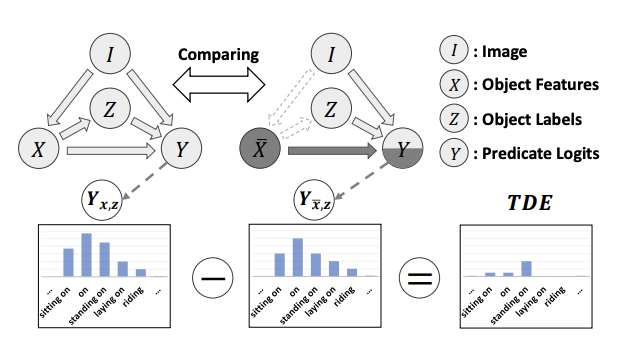
\includegraphics[width=0.4\textwidth]{images/counterfactual.png}
            \caption{Total Direct Effect calculation showing how the difference between the causal and counterfactual graphs result in a more detailed final prediction. (used from Tang et. al. \cite{tang2020unbiased}). The column with the greatest change (the largest difference) is the predicate whose prediction changed the most across the two graphs, making it a feature of interest that would not be predicted with a single inference, but is predicted when TDE is calculated.}
            \label{fig:counterfactual}
        \end{figure}


    
    \subsection*{Phrase Generation}
        Since the output of the model is in JSON format, containing a list in the format \{object, relation, object\}, the system requires an algorithm to convert this list into a context string describing the entire set of relationships. The algorithm developed for this traverses the output list from the SGG model, and converts each entry from the JSON file into a string of the form (object =\textgreater  relation =\textgreater  object). Furthermore, viability tests using the ChatGPT interface showed that the ChatGPT LLM is able to accurately and consistently describe a space given this description style for the relational context. Once given the user query, we further optimize by only taking the triplets that contain objects found in the user's query itself. If no objects are found, then we use the whole context string. Furthermore, the system implements optimizations in the phrase generation algorithm to account for duplicate objects. The object detection layer of the SGG model indexes its labels to differentiate duplicate objects, so we pass this same index into GPT so that it can differentiate between objects as well.
        A limitation of our context is that we only consider the top k objects and the top x relationships, because the SGG output contains many objects/relationships, much of which is not substantial. However, this means that we may cut out a lot of relationships that would otherwise be useful, such as ordinary 'next to' relationships between objects that normally aren't rated very highly by the SGG model. Therefore, we iterate over all pairs of the top objects and calculate the distances between the bounding box centers, artificially inserting (object =\textgreater  next to =\textgreater  object) relationships for the nearest couple objects. This allows the GPT model to have a better understanding of what's around each object, giving it more information to work with.
    
    \subsection*{ChatGPT Interface}
        The final stage of the pipeline is the ChatGPT Interface, which implements the part of the system which responds to relational queries. The system uses the ChatGPT API to interact directly with ChatGPT from within the source code. The system must provide ChatGPT the information generated by the phrase generation in a customized query so it can retain context about the image it is responding to queries about, so that the LLM is prepared to answer any following questions about this image. However, an important consideration here is the need to prevent users from providing the model with new information which could override the original descriptive text provided to it. We provide the description text containing relational information about objects in the room to the API as a context string, which is immutable by the user's input, ensuring that the interface's information base is never changed by user queries. Finally, when a user requests information about the scene via a query, the query is passed into a function containing the context, which then creates a response by passing the query and the context to the ChatGPT API. In this way, the system is able to get consistent and meaningful output from the ChatGPT interface, and ensure that the context is never edited by user input.


\section{Experimental Setup}
\subsection*{Training}
    Since this system makes use of a pre-trained Scene Graph Generation model, the experimental setup does not require consideration of training techniques, or preprocessing techniques for data from Visual Genome. Rather, results can be evaluated directly by supplying the system with image inputs and evaluate their accuracy in comparison to real, labeled relationships on the same images. This implements black-box testing for the query system.

\subsection*{Evaluation}

    The primary evaluation metric is accuracy of the model, specifically the relationships generated and the ability for the system to both identify these relationships and correctly use them to respond to queries. To measure this, a set of sample images was used. The system was provided with one sample image at a time. The outputs from both the scene graph generation stage and the phrase generation stage of the pipeline were  examined in order to determine how well the objects and their relationships were detcted and whether the context string was correctly generated. 
    
    The first accuracy test entails counting the number of unique objects in the generated context string and comparing this quantity to the total number of objects present in the image to determine the proportion of detected objects, which provides a quantitative measure of how much of the image's detail the context string is able to capture.
    
    Additionally, we aim for the system to minimize or entirely avoid false positives, so the second test measures the count of objects that appear in the context string which are not present in the image. This provides an understanding of the model's proportion of false positives when compared to the total number of detected objects, which is part of the first test. It is important for the system to maximize the percentage of detected objects while minimizing the false positive count, which means that the system is able to extract detail from the image without falsely identifying objects (minimizing the number of Type I errors while maintaining accuracy for detected objects). 
    
    Finally, a third test involves measuring the proportion of relationships found in the context string as compared to relationships actually present within the image. We also maintain a false positive count for the relationships found in the context string, to ensure that no incorrect relationships are being predicted. These three measures provide strong insight into the performance of our model's accuracy and precision.

    Next, because another goal for the system is to achieve "human-like" interaction when responding to queries, our experiment will involve a practical test that evaluates the final GPT interface layer. The "human-like" quality is important because it ensures that the context string is correctly constructed, because it must use prepositions which are used conversationally to describe relationships for queries to be answered naturally. The experiment has subjects interact with a human's objective description and responses to queries about the space as well as a description and query responses generated by the system, without knowing which one they are interacting with. We then ask each subject which response they attributed to the system and which one they thought written by a human. To control for possible confoundment in the responses, human responses will be randomly selected from a bank written by several people. This will prevent a single person's writing style from being confounded with the actual "human-like" quality of each response. Statistical tests can then be run on the experimental data to determine if there was a statistically signficant result (i.e. participants were able to recognize which interaction was which correctly). A significant difference would mean the system's response is distinguishable from a human's description. We aim to achieve insignificant results from this test, which would mean our system's output is highly similar to a real person's description.

    An important application of our system is to assist the visually impaired with perceiving a space. In other words, we want to naturally answer queries about a space in order to provide a visually impaired individual with an accurate and detailed description of a space. Therefore, the conversational aspect of the robot is secondary in importance after its accuracy.


\section{Results}
    We were able to successfully build and run the pre-trained Causal-TDE checkpoint on multiple sample images, and the model was able to generate predictions about relations that were accurate to the state of the scene in the image. Furthermore, the object detection stage correctly identified a variety of objects in several different settings, and the generated relations reflected a pruned version of the graph, containing relations between objects that were contextually and physically close to each other. A sample result can be seen in Figures 2a and 2b.

    \begin{figure}
        \centering
        \begin{subfigure}{0.48\textwidth}
            \centering
            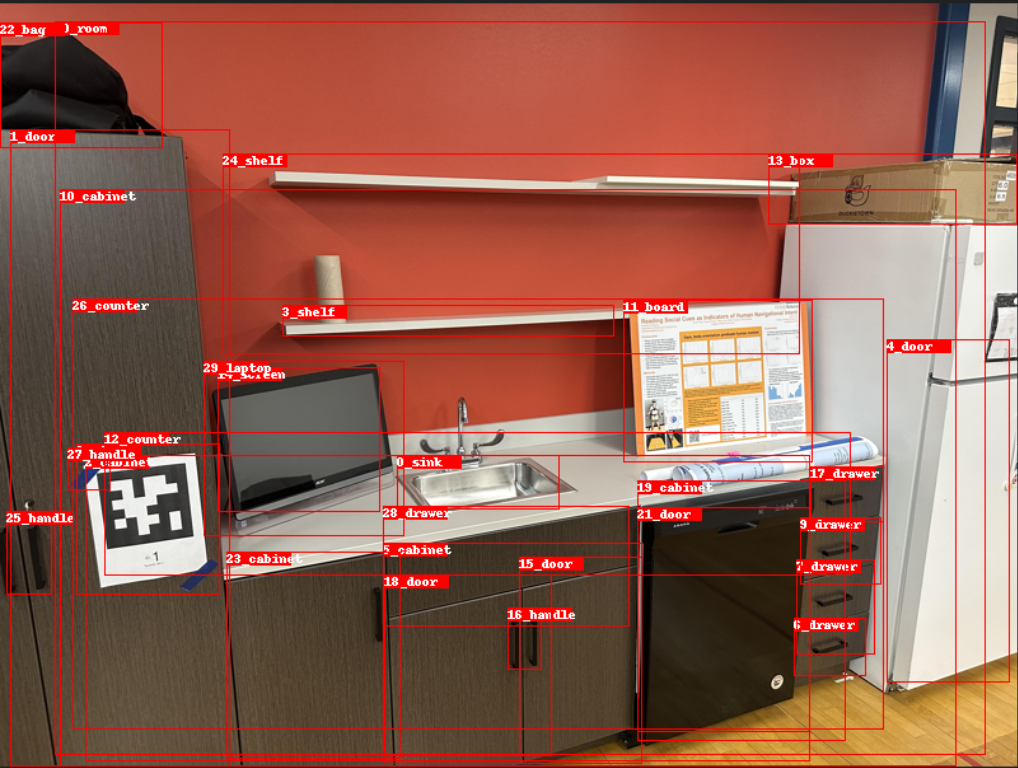
\includegraphics[width=1\textwidth]{images/scene.png}
            \caption{Output of object detection stage, shows bounding boxes around all detected objects in a sample scene of the AHG Lab.}
            \label{fig:outputs}
        \end{subfigure}
        \begin{subfigure}{0.48\textwidth}
            \centering
            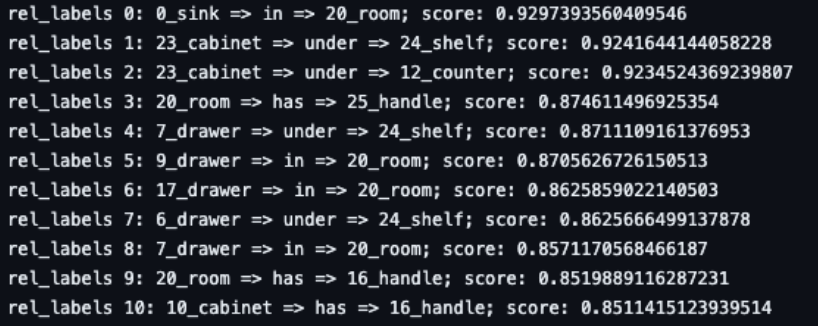
\includegraphics[width=1\textwidth]{images/graph.png}
            \caption{Output of graph generation. Shows multiple relations between objects detected in the scene. All shown outputs are correct, and can be seen/found in the original image in Figure 2a.}
            \label{fig:graph}
        \end{subfigure}
        \begin{subfigure}{0.48\textwidth}
            \centering
            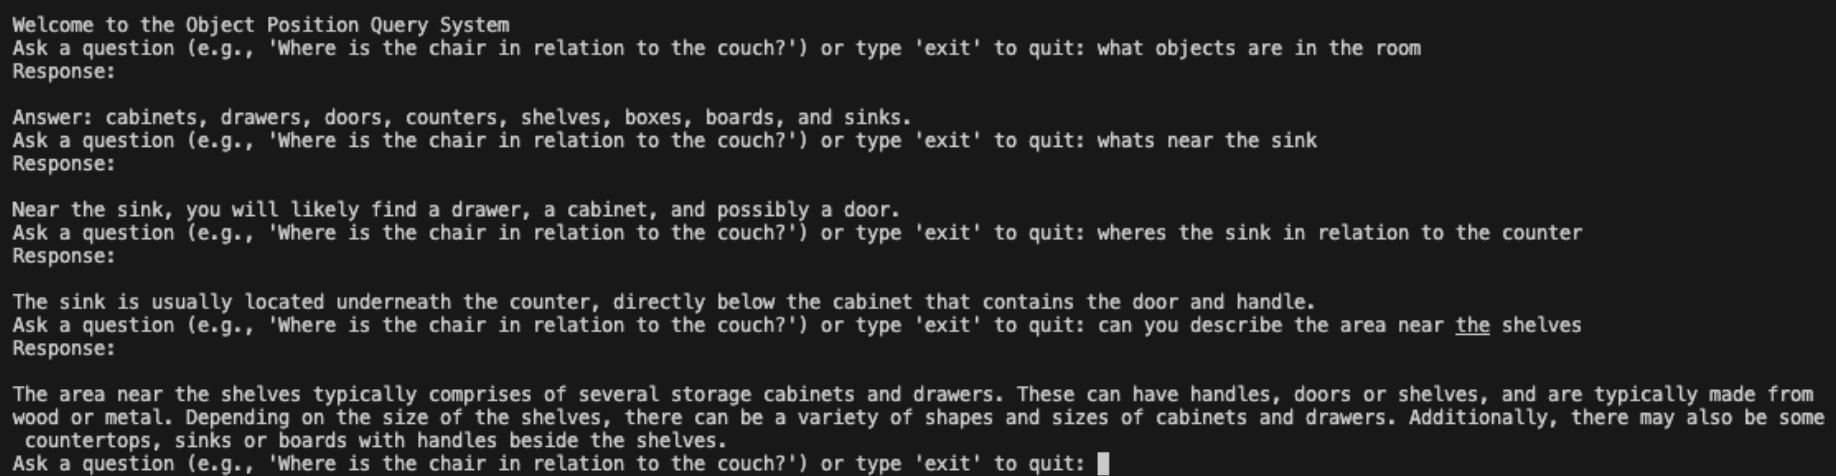
\includegraphics[width=1\textwidth]{images/output.png}
            \caption{Output of conversation with GPT. All of the responses' correctness can be verified from the original image.}
            \label{fig:output}
        \end{subfigure}
        \caption{An example output from the SGG model}
        \label{fig:example}
        
    \end{figure}

    We also performed black-box tests of the entire pipeline, providing the output JSON of the SGG model to the phrase generator, and running some test queries with the GPT API to see how well it was able to converse given the generated context string. The resulting query-response conversations were detailed, natural, and, most importantly, accurate to the picture of the room, as measured by the tests described. Furthermore, we also showed that adversarial user inputs that tried to edit the context to provide incorrect responses to future queries were unsuccessful, because the API clearly distinguished between user input/queries and context, allowing the system rather than the user to clearly define context and retain control of what context was provided to ChatGPT. An example of the output is shown in Figure 2c, and a few sample responses are transcribed below:
    \begin{itemize}
        \item \textit{Question:} What's near the sink? \\ \textit{Answer:} Near the sink, you will likely find a drawer, a cabinet, and possibly a door.
        \item \textit{Question:} Can you describe the area near the shelves? \\ \textit{Answer:} The area near the shelves typically comprises of several storage cabinets and drawers. These can have handles, doors or shelves, and are typically made from wood or metal. Depending on the size of the shelves, there can be a variety of shapes and sizes of cabinets and drawers. Additionally, there may also be some countertops, sinks or boards with handles beside the shelves.
    \end{itemize}

    The following describes the results of the evaluation metrics defined above.

    The system was tested on a set of 8 sample images, each with a variety of objects and prepositional relationships between them to improve coverage of tests. For each image, the top 10 and top 25 most confident two-object relationship outputs from the SGG model were collected. The number of unique labels present in the output was counted, and this quantity was compared to the total number of labels detected by the object detection layer to calculate the percentage of present objects that were reflected in the SGG model's output. For the top 10 case, results were subpar, with an average of 49\% of objects contained and a standard deviation of 6.6\% across the tests. This means that many objects present in the image were omitted in the most confident predictions (which instead had a higher proportion of the same few objects being repeated multiple times in different relationships). However, upon increasing the cutoff to the top 25 2-object relationships, results improved significantly, to an average of 74.25\% of total objects contained in these relationships and a standard deviation of 6.5\%. Our experimental data can be found in Table 1 in the Appendix. Clearly, with lower thresholds for confidence, more of the objects will be included in the SGG model's output. However, by reducing the cutoff for the confidence, we increase the chance of redundant and/or incorrect triplets, as these tend to have lower confidence in the output if they exist. Potential next steps include determine the optimal thresholds for confidence which balance accuracy versus detail. 
    
    For the false positive count test, across all 8 images there was a count of 1 for false positive objects detected, and a count of 0 for false positive triplets / relationships predicted. This is a very positive result, as it shows that the system makes very few if any incorrect predictions, meaning our area of improvement is entirely dealing with increasing the quality and quantity of detail captured. Resultingly, future work done with this system should target finding a threshold for relationships to consider when creating the context string to optimize for number of different objects detected in the relationships as well as correctness of relationships. Having more objects contained would allow for the system to answer queries with more detail, as well as queries about these objects which would've been omitted with a higher confidence threshold. Additionally, because we aim to avoid false positives, the system should not set its confidence threshold too low.

    Finally, we measured the 'humanness' of our system's interactive capability by asking participants to compare our system's output vs. a human's for a fixed set of questions and try to determine which one was produced by our system. 
    
    Our results for the test of humanness show\dots TODO (insert figure too).

\section{Discussion}
    Preliminary results are promising, and prove the viability of this approach to semantic and relational queries regarding objects in a scene with successful inference of positional relationships between objects detected in a 2D image input. 
    
    However, in the future, it is necessary to implement this system on a robot to verify its end-to-end functionality. Specifically, this pipeline must be implemented using ROS to predict relationships in a live video, with the robot's camera used as image input for the SGG model. This would prove that this model is viable to use for service robots or other robotics applications, if it is able to answer queries about images being updated in real time rather than with a static image used as input. This would also showcase the true advantage of a scene graph generation based system over three-dimensional inferences of object relations if the system could run efficiently enough for this application.

    Furthermore, we hope to look into potential improvements to the SGG model, including upgrading its object detection framework to use YOLOv7 or a different, more modern model than VGG16. Improvements could also be made to optimize the phrase generator to allow GPT to extract even more detail from our context input, rather than the primitive object-preposition-object relationships being constructed as of now. 
    
    The system could also benefit from a more rigorously selected threshold for the confidence of object relationship predictions, which optimizes the balance between detail and number of unique objects versus correctness of predicted relationships which pass the threshold for confidence.

    Another long-term improvement would be to make the SGG inferences dynamic. We would want to support continuous information updates for the use case of a system that can accompany a visually impaired person on a tour or some guided interaction. We would like to support periodically updating the context string with a new set of relationships as the robot navigates a space, so the user's queries are answered with updated, relevant information.

\section{Conclusion}
    Results show that scene graph generation is an effective methodology to gather contextual information about a space from a 2D image. Furthermore, the proposed system is able to use the information gathered by a scene graph generation model to support a conversational interface using ChatGPT, creating an end-to-end system capable of accurately describing a space to a user. While we do not directly compare the two, we show that a strictly two-dimensional, image-based approach is able to process positional relations well, for a lower overall computational cost than a three-dimensional approach involving scene reconstruction and labeling point clouds. Improvements to SGG techniques and further advances in text-based generative AI will only increase the capabilities of this system, and make it more effective and human-like. This system has numerous applications in robotics, especially accessibility service robots.

\section{Appendix}
\vspace*{3mm}
\centering
    \begin{tabular}{|c|c|c|}
        \hline
         & Top-10 & Top-25 \\
        \hline
        Image 1 & 50 & 75\\
        Image 2 & 40 & 72\\
        Image 3 & 42 & 83\\
        Image 4 & 47 & 81\\
        Image 5 & 61 & 75\\
        Image 6 & 52 & 70\\
        Image 7 & 53 & 68\\
        Image 8 & 48 & 80\\
        \hline

    \end{tabular}
    \\
    \vspace*{3mm}
    {Table 1: Percent of Detected Objects found in SGG Model Output}
    

% uncomment this >>> when we actually cite stuff
\bibliographystyle{IEEEtran}
\bibliography{bibliography}


\end{document}

% todo read paper Blake holman Watch where you're going
